\documentclass{article}
\usepackage{graphicx}
\usepackage{natbib}
\usepackage{wrapfig}
\usepackage{amsmath, amssymb, amsthm}
\usepackage[utf8]{inputenc}
\usepackage{tikz}

\title{Geometry: Introduction}
\author{TSS Math Club}
\date{December 5 2023}

\begin{document}

\maketitle

\section{Definitions}

    \subsection{General Symbols and Notation}
    
        \subsubsection{Points and Lines}
            \begin{itemize}
                \item \textit{A}
                \item $\overline{AB}$
                \item $\overrightarrow{AB}$
                \item $\overleftrightarrow{AB}$
                \item \textit{AB}
                \item $A \perp B$
                \item $A \parallel B$
                \item Hashmarks, Feathers, Arcs
            \end{itemize}
            
        \subsubsection{Angles}
            \begin{itemize}
                \item $\angle A$
                \item $\measuredangle A$
                \item $\sphericalangle A$
                \item $A ^\circ$
                \item \textit{A} rad
                \item $A \cong B$
            \end{itemize}

    \subsection{Angles}
        \begin{itemize}
            \item Right
            \item Acute
            \item Obtuse
            \item Straight
            \item Reflex
            \item Opposite
            \item Complementary
            \item Supplementary
        \end{itemize}
        
    \subsection{Shapes and Polygons}
    
        \subsubsection{Shape}
            \begin{itemize}
                \item Form/outline/boundary of an object
            \end{itemize}
            
        \subsubsection{Polygon}
            \begin{itemize}
                \item Shape formed by line segments connected at vertices
                \item Simple Polygon: Polygon formed by non-intersecting line segments connected end-to-end
                \item Complex Polygon: Self-intersecting polygon formed by intersecting line segments, which create multiple interior regions
                \item Examples:
                \begin{itemize}
                    \item Pentagon: Simple polygon with five edges and five vertices
                    \item Star: Complex polygon with ten edges and ten vertices
                \end{itemize}
            \end{itemize}

\section{Basic Geometry}

    \subsection{Parallelism}

        \subsubsection{Definition}
            \begin{itemize}
                \item Two lines that share an equidistant separation throughout their entire length are parallel.
                \item Parallel lines do not intersect each other.
            \end{itemize}

        \subsubsection{Properties}
        
            % Diagram
            \tikzset{every picture/.style={line width=1pt}}   
            \begin{tikzpicture}[x=0.75pt,y=0.75pt,yscale=-1,xscale=1]
            \hspace{20pt}
            
            % Parallel Lines
            \draw    (100,100) -- (400,100);
            \draw    (100,200) -- (400,200);
            
            % Diagonal/Transverse Line
            \draw    (180, 55) -- (300,245) ;
            
            % Angles a, b, c, d
            \draw (185, 86) node [anchor=north west][inner sep=0.75pt]   [align=left] {a};
            \draw (208, 82) node [anchor=north west][inner sep=0.75pt]   [align=left] {b};
            \draw (197,107) node [anchor=north west][inner sep=0.75pt]   [align=left] {c};
            \draw (221,103) node [anchor=north west][inner sep=0.75pt]   [align=left] {d};

            % Angles e, f, g, h
            \draw (249,186) node [anchor=north west][inner sep=0.75pt]   [align=left] {e};
            \draw (272,182) node [anchor=north west][inner sep=0.75pt]   [align=left] {f};
            \draw (259,207) node [anchor=north west][inner sep=0.75pt]   [align=left] {g};
            \draw (285,203) node [anchor=north west][inner sep=0.75pt]   [align=left] {h};
            
            \end{tikzpicture}
            
            \begin{itemize}
                \item Corresponding angles are equal (PLT-F): $\angle \text{a} = \angle \text{e}$
                \item Alternate interior angles are equal (PLT-Z): $\angle \text{d} = \angle \text{e}$
                \item Consecutive interior angles are supplementary (PLT-C): $\angle \text{c} +\angle \text{e} = 180^{\circ}$
            \end{itemize}
            
            \begin{tikzpicture}[x=0.75pt,y=0.75pt,yscale=-1,xscale=1]
            
            % Parallel Lines
            \draw    (100,100) -- (400,100);
            \draw    (100,150) -- (400,150);
            \draw    (100,200) -- (400,200);
            
            % Diagonal/Transverse Line
            \draw    (350, 55) -- (150,245);

            % Labels
            \draw ( 85, 92) node [anchor=north west][inner sep=0.75pt]   [align=left] {A};
            \draw (400, 92) node [anchor=north west][inner sep=0.75pt]   [align=left] {B};
            \draw ( 85,142) node [anchor=north west][inner sep=0.75pt]   [align=left] {C};
            \draw (400,142) node [anchor=north west][inner sep=0.75pt]   [align=left] {D};
            \draw ( 85,192) node [anchor=north west][inner sep=0.75pt]   [align=left] {E};
            \draw (400,192) node [anchor=north west][inner sep=0.75pt]   [align=left] {F};
            
            \end{tikzpicture}
            
            \begin{itemize}
                \item Parallelism is a transitive property
                \item $\overline{AB} \parallel \overline{CD}$ and $\overline{CD} \parallel \overline{EF} \implies \overline{AB} \parallel \overline{EF}$
                \item All parallel angle theorems will hold true for the angles of the intersections of all parallel lines and a transversal.
            \end{itemize}
        
        \subsubsection{Example Problem}
            \hspace{20pt}
            \begin{tikzpicture}[x=0.75pt,y=0.75pt,yscale=-1,xscale=1]
            
            % Lines
            \draw    (110,100) -- (420,100);
            \draw    (110,240) -- (420,240);
            \draw    (200, 60) -- (150,280);
            \draw    (165, 75) -- (360,265);
            \draw    (123, 265) -- (402, 75);
            
            % Labels
            \draw (193,84) node [anchor=north west][inner sep=0.75pt]   [align=left] {A};
            \draw (355,84) node [anchor=north west][inner sep=0.75pt]   [align=left] {B};
            \draw (158,243) node [anchor=north west][inner sep=0.75pt]   [align=left] {C};
            \draw (324,243) node [anchor=north west][inner sep=0.75pt]   [align=left] {D};
            \draw (256,151) node [anchor=north west][inner sep=0.75pt]   [align=left] {E};
            
            \end{tikzpicture}
            
            \begin{minipage}{.8\linewidth}
            Given $\overline{AB} \parallel \overline{CD}$, $\overline{AE}$ bisects $\angle BAC$, $\overline{CE}$ bisects $\angle ACD$
            Prove $\overline{AE} \perp \overline{CE}$
            \end{minipage}
            
    \subsection{Triangles}
    
        \subsubsection{Definition}
            \begin{itemize}
                \item A simple polygon with three edges and three vertices
            \end{itemize}
            
        \subsubsection{Classifications}
            \begin{itemize}
                \item Equilateral
                \item Isosceles
                \item Scalene
                \item Acute
                \item Obtuse
            \end{itemize}

        \subsubsection{Properties}
            \begin{itemize}
                \item Angles: Sum of angles in any triangle is 180$^\circ$
                \item Sides: The length of any side is less than the sum and more than the difference of the length of the other two sides
            \end{itemize}

        \subsubsection{Triangle Inequality Theorem}
            \begin{itemize}
                \item The sum of the lengths of any two sides in any triangle must be greater than the length of the third side
            \end{itemize}

        \subsubsection{Pythagorean Theorem}
            \hspace{40pt}
            \begin{tikzpicture}[x=0.75pt,y=0.75pt,yscale=-1,xscale=1]
            
            % Parallel Lines
            \draw    (100,100) -- (100,230);
            \draw    (100,230) -- (230,230);
            \draw    (100,100) -- (230,230);

            % Labels
            \draw ( 85,162) node [anchor=north west][inner sep=0.75pt]   [align=left] {a};
            \draw (158,233) node [anchor=north west][inner sep=0.75pt]   [align=left] {b};
            \draw (167,157) node [anchor=north west][inner sep=0.75pt]   [align=left] {c};

            \end{tikzpicture}
            
            \begin{itemize}
                \item $a^2 + b^2 = c^2$
            \end{itemize}

        \subsubsection{Exterior angle theorem}   
            
            \begin{tikzpicture}[x=0.75pt,y=0.75pt,yscale=-1,xscale=1]
            
            % Lines
            \draw    (109.72,221.16) -- (424.72,221.16);
            \draw    (224.72,98.16) -- (109.72,221.16);
            \draw    (224.72,98.16) -- (275.72,220.16);
            
            % Labels
            \draw (103,225) node [anchor=north west][inner sep=0.75pt]   [align=left] {A};
            \draw (270,225) node [anchor=north west][inner sep=0.75pt]   [align=left] {B};
            \draw (216, 79) node [anchor=north west][inner sep=0.75pt]   [align=left] {C};
            \draw (122,204) node [anchor=north west][inner sep=0.75pt]   [align=left] {a};
            \draw (253,202) node [anchor=north west][inner sep=0.75pt]   [align=left] {b};
            \draw (217,114) node [anchor=north west][inner sep=0.75pt]   [align=left] {c};
            \draw (279,203) node [anchor=north west][inner sep=0.75pt]   [align=left] {d};
            
            \end{tikzpicture}
        
        \subsubsection{Congruence and Similarity}
            \begin{itemize}
                \item Congruent Triangles: Same angles and same size
                \subitem proven by SSS, SAS, ASA, AAS
                    \subitem ambiguous case SSA
                \item Similar Triangles: Same angles
                    \subitem proven by AA
            \end{itemize}

        \subsubsection{Perimeter and Area}
            \begin{itemize}
                \item Perimeter: Sum of lengths of all sides
                \item Area: For right triangles: $\frac{1}{2} \cdot$ base $\cdot$ height
                    \subitem For all triangles: Heron's formula
            \end{itemize}

        \subsubsection{Example Problems}
            \includegraphics[scale=0.7]{2015AMC10AProblem19Picture.png}\\
            Given $\bigtriangleup ABC$ is an isosceles right triangle, $\overline{CD}$ and $\overline{CE}$ trisect $\angle ACB$\\
            Find the area of $\bigtriangleup CDE$\\
            \includegraphics[scale=0.6]{20221013_Q.png}\\
            Points \textit{S} and \textit{T} are on sides \textit{QR} and \textit{PQ} of $\bigtriangleup PQR$ respectively, such that $\overline{PS} \perp \overline{QR}$, and $\overline{RT} \perp \overline{PQ}$.\\
            Given $PT=1$, $TQ=4$, $QS=3$\\
            Find the length of $SR$.

    \subsection{Quadrilaterals}
    
        \subsubsection{Definition}
            \begin{itemize}
                \item A simple polygon with four edges and four vertices
            \end{itemize}
            
        \subsubsection{Classifications}
            \begin{itemize}
                \item Rectangle
                    \subitem Square
                \item Parallelogram
                    \subitem Rhombus
                \item Trapezoid
                    \subitem Acute, Right, Obtuse, Isosceles
                \item Kite
                \item Scalene
                \item Cyclic
            \end{itemize}

        \subsubsection{Congruence and Similarity}
            \begin{itemize}
                \item Congruent Quadrilaterals: Same angles and same size
                \item Similar Quadrilaterals: Same angles
            \end{itemize}

        \subsubsection{Perimeter and Area}
            \begin{itemize}
                \item Perimeter: Sum of lengths of all sides
                \item Area: Different formulae for different quadrilaterals
                \subitem \textit{e.g.} length $\cdot$ width for rectangles, base $\cdot$ height for parallelograms
            \end{itemize}
    
    \subsection{Circles}
    
        \subsubsection{Definition}
            \begin{itemize}
                \item A closed curve in which all points are equidistant from the center
            \end{itemize}
        
        \subsubsection{Geometric objects related to circles}

            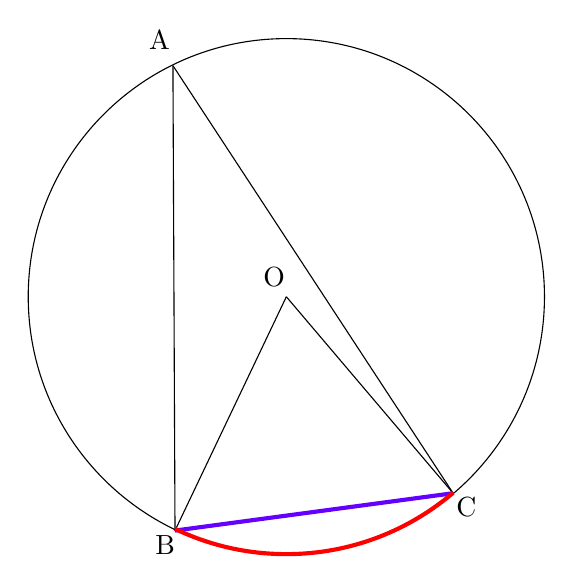
\begin{tikzpicture}[x=0.75pt,y=0.75pt,yscale=-1,xscale=1]
            
            % Circle
            \draw   (28,148.36) .. controls (28,79.68) and (83.68,24) .. (152.36,24) .. controls (221.04,24) and (276.72,79.68) .. (276.72,148.36) .. controls (276.72,217.04) and (221.04,272.72) .. (152.36,272.72) .. controls (83.68,272.72) and (28,217.04) .. (28,148.36) -- cycle;
            
            % Lines
            \draw    (152.36,148.36) -- (232.72,243.03);
            \draw    (152.36,148.36) -- (98.72,261.03);
            \draw    (97.72,37.03) -- (98.72,261.03);
            \draw    (97.72,37.03) -- (232.72,243.03);
            
            % Chord
            \draw [color={rgb, 255:red, 100; green, 0; blue, 255 }  ,draw opacity=1 ][line width=1.5]    (98.72,261.03) -- (232.72,243.03);
            
            % Arc
            \draw  [draw opacity=0][line width=1.5]  (232.73,242.82) .. controls (211.08,261.25) and (183.02,272.38) .. (152.36,272.38) .. controls (133.15,272.38) and (114.96,268.01) .. (98.72,260.21) -- (152.36,148.36) -- cycle;
            \draw  [color={rgb, 255:red, 255; green, 0; blue, 0 }  ,draw opacity=1 ][line width=1.5]  (232.73,242.82) .. controls (211.08,261.25) and (183.02,272.38) .. (152.36,272.38) .. controls (133.15,272.38) and (114.96,268.01) .. (98.72,260.21);  
            
            % Points
            \draw (140,133) node [anchor=north west][inner sep=0.75pt]   [align=left] {O};
            \draw (85,19) node [anchor=north west][inner sep=0.75pt]   [align=left] {A};
            \draw (88,262) node [anchor=north west][inner sep=0.75pt]   [align=left] {B};
            \draw (233,244) node [anchor=north west][inner sep=0.75pt]   [align=left] {C};
        
        
            \end{tikzpicture}
            
            \begin{itemize}
                \item Center: Center of the circle, Point O
                \item Radius: Length from center to circumference.
                \item Arc: A curve that lies on the circumference of a circle.
                \item Chord: A straight line between two points on a circle.
                \item Central angle: Angle formed at the center of a circle by two radii
                    \subitem $\angle BOC$ is a central angle.
                \item Inscribed angle: Angle formed inside the a circle by two chords
                    \subitem $\angle BAC$ is an inscribed angle.
            \end{itemize}

        \subsubsection{Circumference and Area}
            \begin{itemize}
                \item Circumference: $2 \cdot \pi \cdot r$
                \item Area: $\pi \cdot r^2$
            \end{itemize}
            
% \section{Derivations}
% \begin{itemize}
%     \item Angle sum in a triangle.
%     \item Triangle area formula.
%     \item Heron's formula.
% \end{itemize}
    
\end{document}
